\documentclass[multi=tikzpicture,border=7pt]{standalone}
\usepackage{ctex,amsmath,bm}
\usepackage{tikz}
\usetikzlibrary{arrows.meta,calc,angles,quotes,decorations.pathmorphing,patterns,positioning}
\tikzset{
  axis/.style={->,>=Stealth,thick},
  force/.style={->,>=Stealth,very thick},
  flow/.style={->,>=Stealth,thick,blue!70!black},
  dim/.style={<->,>=Stealth,thin},
  body/.style={draw=black,fill=blue!9,thick},
  point/.style={circle,fill=black,inner sep=1.6pt}
}
\begin{document}

% 01 question-01
\begin{tikzpicture}[x=.9cm,y=.9cm]
\draw[axis](-3.3,0)--(3.3,0) node[right]{$x$};\draw[axis](0,-1.8)--(0,3.4) node[above]{$y$};
\draw[body](0,0)ellipse[x radius=2.25,y radius=1.25];
\pgfmathsetmacro{\rr}{sqrt(2.25^2+1.25^2)}
\draw[very thick](-3.3,\rr-3.3)--(0,\rr)--(3.3,\rr-3.3);
\fill(0,\rr)circle(2pt) node[above right]{$M$};\node[below right]at(0,0){$O$};
\draw[dim](0,0)--(0,\rr)node[midway,right]{$\rho$};\node at(0,-2.1){两直角边为真实切线};
\begin{scope}[shift={(8,0)}]
\pgfmathsetmacro{\cx}{sqrt(1.1^2*cos(20)^2+1.85^2*sin(20)^2)}
\pgfmathsetmacro{\cy}{sqrt(1.1^2*sin(20)^2+1.85^2*cos(20)^2)}
\draw[axis](-.2,0)--(3.4,0)node[right]{$x$};\draw[axis](0,-.2)--(0,4.1)node[above]{$y$};
\draw[body,rotate around={20:(\cx,\cy)}](\cx,\cy)ellipse[x radius=1.1,y radius=1.85];
\draw[dashed](2.1523,0)arc[start angle=0,end angle=90,radius=2.1523];
\draw[dim](0,0)--(\cx,\cy)node[midway,left]{$\rho$};\fill(\cx,\cy)circle(2pt)node[right]{$C$};
\node[align=center]at(1.5,-.7){中心距离由支撑函数确定\\两处确实与坐标轴相切};
\end{scope}
\end{tikzpicture}

% 02 solution-01
\begin{tikzpicture}[x=.9cm,y=.9cm]
\draw[axis](-3.2,0)--(3.2,0)node[right]{$x$};\draw[axis](0,-1.8)--(0,3.3)node[above]{$y$};
\draw[body](0,0)ellipse[x radius=2.25,y radius=1.25];
\pgfmathsetmacro{\ha}{sqrt(2.25^2*cos(30)^2+1.25^2*sin(30)^2)}
\pgfmathsetmacro{\hb}{sqrt(2.25^2*cos(120)^2+1.25^2*sin(120)^2)}
\pgfmathsetmacro{\mx}{\ha*cos(30)+\hb*cos(120)}\pgfmathsetmacro{\my}{\ha*sin(30)+\hb*sin(120)}
\coordinate(M)at(\mx,\my);
\draw[very thick](M)--++(4*.5,-4*.8660254);\draw[very thick](M)--++(-4*.8660254,-4*.5);
\draw[dashed,red!70!black](0,0)circle(2.57391);\fill(M)circle(2pt)node[above right]{$M$};
\draw[dim](0,0)--(M)node[midway,left]{$\rho$};
\node at(0,-3){$\bm r_M=h_1\bm n_1+h_2\bm n_2$};
\begin{scope}[shift={(8,0)}]
\draw[thick](0,0)circle(2.3);\coordinate(P)at(55:2.3);\fill(P)circle(3pt)node[left]{$m$};
\draw[dashed](0,0)--(0,2.3);\draw(0,0)--(P);
\draw[->](0,.8)arc[start angle=90,end angle=55,radius=.8]node[midway,right]{$\theta$};
\draw[force,red!75!black](P)--++(55:1.3)node[right]{$N$};
\draw[force](P)--++(0,-1.5)node[right]{$mg$};
\node[align=center]at(0,-3){$N$ 沿圆外；向心方程\\$mg\cos\theta-N=mv^2/\rho$};
\end{scope}
\end{tikzpicture}

% 03 question-02
\begin{tikzpicture}[x=1cm,y=1cm]
  \draw[very thick] (-.7,0)--(8.8,0);
  \draw[fill=blue!12,thick] (0,0) rectangle (7.5,.35);
  \filldraw[fill=orange!25,thick] (.7,1.28) circle(.42);
  \coordinate (Qi) at (-.15,2.25);
  \coordinate (Qp) at (.7,1.28);
  \coordinate (Qv) at (.7,2.5);
  \draw[flow] (-.15,2.25)--(.55,1.58) node[midway,left]{$v_0$};
  \draw[dashed] (.7,1.3)--(.7,2.65);
  \draw pic[draw,->,"$\theta$",angle radius=.58cm,angle eccentricity=1.35]
    {angle=Qv--Qp--Qi};
  \node at (.7,.68){$m$};
  \node at (4.3,.15){木板，$m$};
  \draw[dim] (0,-.45)--(7.5,-.45) node[midway,below]{$l$};
  \node at (4.2,-1.25){地面光滑，球—板间动摩擦因数为 $\mu$};
\end{tikzpicture}

% 04 solution-02
\begin{tikzpicture}[x=.9cm,y=.9cm]
  \begin{scope}
    \draw[very thick] (-.5,0)--(5.7,0);
    \draw[fill=blue!10,thick] (0,0) rectangle (5,.3);
    \filldraw[fill=orange!24,thick] (1.15,.82) circle(.5);
    \draw[force,red!75!black] (1.15,.32)--++(0,1.45) node[above left]{$J_y$};
    \draw[force,blue!70!black] (1.15,.32)--++(-1.35,0) node[above]{$J_x$};
    \draw[flow] (.6,2.05)--(1.8,2.05) node[midway,above]{$v_x'$};
    \draw[flow] (3.0,.7)--(4.4,.7) node[midway,above]{$V$};
    \node at (2.55,-.55){质点模型：碰撞冲量};
  \end{scope}
  \begin{scope}[shift={(7.1,0)}]
    \draw[very thick] (-.5,0)--(5.7,0);
    \draw[fill=blue!10,thick] (0,0) rectangle (5,.3);
    \filldraw[fill=orange!24,thick] (1.15,.82) circle(.5);
    \draw[->,>=Stealth,very thick,purple!75!black]
      (1.62,1.02) arc[start angle=22,end angle=-70,radius=.55] node[below right,xshift=6pt]{$\omega'$};
    \draw[flow] (1.15,.3)--++(1.45,0) node[above right,yshift=20pt]{$v_C'=v_x'-\omega'r$};
    \draw[flow] (3.0,.7)--(4.4,.7) node[midway,above]{$V$};
    \node[align=center] at (2.55,-.65){刚体模型：接触点相对速度\\决定第二次碰撞的摩擦方向};
  \end{scope}
\end{tikzpicture}

% 05 question-03
\begin{tikzpicture}[x=.88cm,y=.88cm]
  \begin{scope}
    \draw[body,fill=gray!10] (-2,-1.35) rectangle (2,1.35);
    \draw[fill=white,thick] (0,0) ellipse[x radius=1.25,y radius=.22];
    \draw[force] (-1.6,-.8)--(-1.6,.75) node[left]{$\bm M$};
    \draw[dim] (1.55,-.22)--(1.55,.22) node[right]{$h$};
    \draw[dim] (-1.25,.52)--(1.25,.52) node[midway,above]{$2R$};
    \node at (0,-1.8){(a) 薄圆盘形洞};
  \end{scope}
  \begin{scope}[shift={(6.1,0)}]
    \draw[body,fill=gray!10] (-2,-1.35) rectangle (2,1.35);
    \draw[fill=white,thick] (-.3,-1.05) rectangle (.3,1.05);
    \draw[force] (-1.5,-.8)--(-1.5,.75) node[left]{$\bm M$};
    \draw[dim] (.58,-1.05)--(.58,1.05) node[midway,right]{$l$};
    \node at (0,-1.8){(b) 长直棒形洞};
  \end{scope}
  \begin{scope}[shift={(12.2,0)}]
    \draw[body,fill=gray!10] (-2,-1.35) rectangle (2,1.35);
    \draw[fill=white,thick] (0,0) circle(.9);
    \draw[force] (-1.55,-.8)--(-1.55,.75) node[left]{$\bm M$};
    \draw[dim] (0,0)--(.78,.45) node[midway,above]{$R$};
    \node at (0,-1.8){(c) 球形洞};
  \end{scope}
\end{tikzpicture}

% 06 solution-03
\begin{tikzpicture}[x=1cm,y=1cm]
\draw[thick](0,0)ellipse[x radius=1.6,y radius=.45];\draw[thick](0,.5)ellipse[x radius=1.6,y radius=.45];
\draw[thick](-1.6,0)--(-1.6,.5)(1.6,0)--(1.6,.5);
\draw[flow](1.6,.5)arc[start angle=0,end angle=-110,x radius=1.6,y radius=.45];
\node[blue!70!black]at(2,.6){$K_b=M$};\draw[force,red!70!black](0,.2)--(0,-1.1)node[right]{$\Delta\bm B$};
\node[align=center]at(0,-1.8){纬向电流：从 $+z$ 看为顺时针\\仅画空腔壁修正场};
\begin{scope}[shift={(6,0)}]
\draw[thick](0,0)circle(1.5);\draw[dashed](-1.5,0)arc[start angle=180,end angle=0,x radius=1.5,y radius=.35];
\draw[flow](1.5,0)arc[start angle=0,end angle=-150,x radius=1.5,y radius=.35];
\draw[force,red!70!black](0,0)--(0,-1.15)node[right]{$\Delta\bm B$};
\draw[force](2,-.5)--(2,1)node[right]{$\bm M$};
\node[align=center]at(0,-2.4){球腔壁电流沿纬圈\\$\Delta\bm B=-2\mu_0\bm M/3$};
\end{scope}
\end{tikzpicture}

% 07 question-04
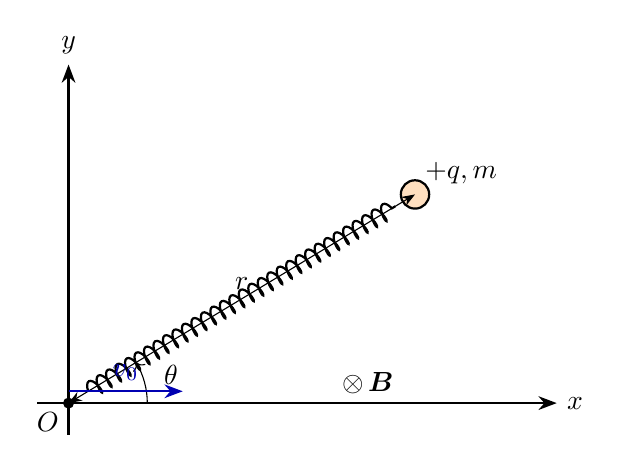
\begin{tikzpicture}[x=1cm,y=1cm]
  \draw[axis] (-.4,0)--(6.2,0) node[right]{$x$};
  \draw[axis] (0,-.4)--(0,4.3) node[above]{$y$};
  \fill (0,0) circle(2pt) node[below left]{$O$};
  \coordinate (P) at (4.4,2.65);
  \coordinate (Ox) at (0,0);
  \coordinate (Xx) at (6,0);
  \filldraw[fill=orange!25,thick] (P) circle(.18) node[above right]{$+q,m$};
  \draw[thick,decorate,decoration={coil,aspect=.35,segment length=4pt,amplitude=3pt}]
    (.25,.15)--(4.15,2.5);
  \draw[dim] (0,0)--(P) node[midway,above]{$r$};
  \draw pic[draw,->,"$\theta$",angle radius=1cm,angle eccentricity=1.35]
    {angle=Xx--Ox--P};
  \draw[flow] (0,.15)--(1.45,.15) node[midway,above]{$v_0$};
  \node at (3.8,.25){$\otimes\,\bm B$};
\end{tikzpicture}

% 08 solution-04
\begin{tikzpicture}[x=.95cm,y=.95cm]
  \begin{scope}
    \draw[axis] (-3.1,0)--(3.4,0) node[right]{$x$};
    \draw[axis] (0,-3.1)--(0,3.4) node[above]{$y$};
    \draw[blue!70!black,very thick] (0,1.7) circle(1.7);
    \fill (0,0) circle(2pt) node[below left]{$O$};
    \draw[force] (0,0)--(1.5,0) node[below]{$v_0$};
    \draw[dim] (0,1.7)--(1.7,1.7) node[midway,above]{$R_c=mv_0/(qB)$};
    \node at (0,-3.65){无弹簧时为过原点的圆};
  \end{scope}
  \begin{scope}[shift={(8.2,0)}]
    \draw[axis] (-3.1,0)--(3.4,0) node[right]{$x$};
    \draw[axis] (0,-3.1)--(0,3.4) node[above]{$y$};
    \draw[red!70!black,very thick,domain=0:180,samples=300,smooth]
      plot ({(2.25*sin(3*\x))*cos(\x)},{(2.25*sin(3*\x))*sin(\x)});
    \draw[dashed] (0,0) circle(2.25);
    \fill (0,0) circle(2pt) node[below left]{$O$};
    \node[align=center] at (0,-3.75){有弹簧时：径向简谐振动\\与匀速转角叠加；示例频率比为 $3$};
  \end{scope}
\end{tikzpicture}

% 09 question-05
\begin{tikzpicture}[x=1cm,y=1cm]
  \draw[very thick] (0,4.8)--(-3.9,-2.1) (0,4.8)--(3.9,-2.1);
  \draw[dashed] (0,4.8)--(0,-2.4);
  \draw[fill=orange!14,thick] (0,3.65) ellipse[x radius=.65,y radius=.18];
  \draw[fill=blue!10,very thick] (0,.2) ellipse[x radius=2.45,y radius=.62];
  \coordinate (Cv) at (0,-1);
  \coordinate (Ca) at (0,4.8);
  \coordinate (Cg) at (3.9,-2.1);
  \draw[dashed] (-2.45,.2) arc[start angle=180,end angle=360,x radius=2.45,y radius=.62];
  \draw[dim] (0,3.65)--(.65,3.65) node[midway,below]{$r_0$};
  \draw[dim] (0,.2)--(2.45,.2) node[midway,above]{$R_0$};
  \draw pic[draw,->,"$\theta$",angle radius=.75cm,angle eccentricity=1.35]
    {angle=Cv--Ca--Cg};
  \draw[flow] (2.2,.75)--(2.85,-.4) node[right]{$v_0$};
  \node[right] at (.75,3.75){固定小环，电流 $I_0$};
  \node[right] at (2.5,.2){导电弹性大环，质量 $m$};
\end{tikzpicture}

% 10 solution-05
\begin{tikzpicture}[x=.9cm,y=.9cm]
  \begin{scope}
    \draw[very thick] (0,4.2)--(-3.2,-1.6) (0,4.2)--(3.2,-1.6);
    \draw[dashed] (0,4.2)--(0,-1.7);
    \draw[thick] (0,.15) ellipse[x radius=2.15,y radius=.5];
    \filldraw[fill=orange!25,thick] (2.15,.15) circle(.16);
    \draw[force] (2.15,.15)--++(0,-1.35) node[right]{$dm\,g$};
    \draw[force,red!75!black] (2.15,.15)--++(-1.3,0) node[above]{$dF_r$};
    \draw[force,blue!70!black] (2.15,.15)--++(-.72,1.25) node[left]{$F_{\rm em}$};
    \draw[dim] (0,.15)--(2.15,.15) node[midway,above]{$R$};
    \node[align=center] at (0,-2.25){母线坐标 $s$：$dR=\sin\theta\,ds$};
  \end{scope}
  \begin{scope}[shift={(7.4,.2)}]
    \draw[axis] (-.3,0)--(5.5,0) node[right]{$R$};
    \draw[axis] (0,-.3)--(0,4.3) node[above]{$M(R)$};
    \draw[blue!70!black,very thick,domain=.7:5,samples=100]
      plot(\x,{3/\x});
    \draw[dashed] (2.2,0)--(2.2,1.365) node[above right]{$R_0$};
    \node[align=center] at (2.7,-1.05){$M(R)=\dfrac{\pi\mu_0r_0^2\sin^3\theta}{2R}$\\运动电势与磁恢复力均由 $dM/dR$ 决定};
  \end{scope}
\end{tikzpicture}

% 11 question-06
\begin{tikzpicture}[x=1cm,y=1cm]
  \draw[very thick] (0,0) rectangle (8,3.2);
  \draw[very thick] (4,0)--(4,3.2);
  \foreach \p in {(.7,.7),(1.2,2.3),(2.0,1.35),(2.8,2.55),(3.25,.75)}
    \fill[blue!70!black] \p circle(2.2pt);
  \foreach \p in {(4.7,.7),(5.2,2.3),(6.0,1.35),(6.8,2.55),(7.3,.75)}
    \fill[red!70!black] \p circle(2.2pt);
  \node[blue!70!black] at (2,3.65){左室：$N$ 个“人”};
  \node[red!70!black] at (6,3.65){右室：$N$ 个“妖”};
  \node at (2,-.45){体积 $v_0/2$，温度 $T_0$};
  \node at (6,-.45){体积 $v_0/2$，温度 $T_1$};
  \draw[flow] (3.25,1.6)--(4.75,1.6) node[midway,above]{抽去隔板};
\end{tikzpicture}

% 12 solution-06
\begin{tikzpicture}[x=.95cm,y=.95cm]
  \begin{scope}
    \draw[thick] (0,0) rectangle (5.4,2.5);
    \draw[dashed] (2.7,0)--(2.7,2.5);
    \foreach \p in {(.5,.5),(1.2,1.8),(2.1,.9),(3.2,1.8),(4.1,.7),(4.8,1.5)}
      \fill[blue!70!black] \p circle(2pt);
    \foreach \p in {(.8,1.25),(1.75,.35),(2.35,2),(3.05,.55),(3.8,1.4),(4.7,.45)}
      \fill[red!70!black] \p circle(2pt);
    \node at (2.7,-.65){可分辨组分各自自由膨胀};
  \end{scope}
  \begin{scope}[shift={(7.3,0)}]
    \node[draw,rounded corners,fill=blue!10,minimum width=1.2cm,minimum height=.65cm] (aa) at (0,1.7){人--人};
    \node[draw,rounded corners,fill=purple!10,minimum width=1.2cm,minimum height=.65cm] (ab) at (2.6,1.7){人--妖};
    \node[draw,rounded corners,fill=red!10,minimum width=1.2cm,minimum height=.65cm] (bb) at (5.2,1.7){妖--妖};
    \draw[<->,>=Stealth,thick] (aa)--(ab);
    \draw[<->,>=Stealth,thick] (ab)--(bb);
    \node[align=center] at (2.6,.3){随机配对概率\\$P_{\text{人人}}:P_{\text{人妖}}:P_{\text{妖妖}}=1:2:1$};
  \end{scope}
\end{tikzpicture}

% 13 question-07
\begin{tikzpicture}[x=1cm,y=1cm]
\draw[fill=blue!6](-3,0)rectangle(4,2.5);\draw[axis](0,-1)--(0,4.4)node[above]{$y$，光轴};\draw[axis](-3,0)--(4.7,0)node[right]{$x$};
\draw[orange!80!black,thick,->](-1.4,-2)--(0,0);\draw[dashed](0,-2)--(0,0);\node at(-.3,-.8){$\theta$};
\draw[blue!70!black,very thick,->](0,0)--(.96,2.5)--(1.94,3.9)node[right]{$o$};
\draw[red!70!black,very thick,->](0,0)--(1.70,2.5)--(2.68,3.9)node[right]{$e$};
\draw[dim](4.3,0)--(4.3,2.5)node[midway,right]{$l$};\node at(1,-2.6){$s,p$等振幅、同相；射线折射示意};
\end{tikzpicture}

% 14 solution-07
\begin{tikzpicture}[x=.85cm,y=.85cm]
\draw[axis](-.5,0)--(6.7,0)node[right]{$x$};\draw[axis](0,-.3)--(0,3.7)node[above]{$y$};
\draw[orange!80!black,thick](0,0)ellipse[x radius=2.8000000,y radius=2.1875000];
\draw[dim](0,0)--(2.8000000,0)node[midway,above]{$c\Delta t/n_e$};\draw[dim](0,0)--(0,2.1875000)node[midway,left]{$c\Delta t/n_o$};
\draw[magenta!70!black,very thick](-.3,2.5830331)--(6.1020638,0)node[below]{$c\Delta t/\sin\theta$};
\coordinate(P)at(1.2848112,1.9436112);\fill(P)circle(2pt);\draw[force,green!55!black](0,0)--(P)node[midway,below right]{$\bm v_g\Delta t$};
\draw[force,blue!70!black](P)--++(0.4588611,1.1372902)node[above]{$\bm k_e$};
\node[align=center]at(2.9,-3.1){法线与切线垂直；切点由色散式计算\\示例：$n_o=1.6,n_e=1.25,\theta=35^\circ$};
\begin{scope}[shift={(10,0)}]
\draw[fill=blue!6](-1,0)rectangle(4,2);\node[left]at(-1,1){$l$};
\draw[blue!70!black,very thick,->](-0.7002075,-1)--(0,0)--(0.7680165,2)--(1.7483070,3.4);
\draw[red!70!black,very thick,->](-0.7002075,-1)--(0,0)--(1.3220866,2)--(2.3023772,3.4);
\draw[dashed](-.3,2.7)--(3,2.7-3.3*0.7002075)node[right]{同一出射波面};
\node[blue!70!black]at(0.7680165,2.25){$o$};\node[red!70!black]at(1.3220866,2.25){$e$};
\node at(1.4,-1.8){出射到空气后方向平行};
\end{scope}\end{tikzpicture}

% 15 question-08
\begin{tikzpicture}[x=1cm,y=1cm]
\draw[axis](-4.6,0)--(4.2,0)node[right]{$x$};\draw[axis](0,-3.5)--(0,3.5)node[above]{$y$};
\draw[thick](0,-3)arc[start angle=-90,end angle=90,radius=3];
\foreach \a in {-90,-60,...,90}{\filldraw[fill=blue!12]({3*cos(\a)},{3*sin(\a)})circle(.1);}
\draw[flow](-2,-2.46)--(0,-3)node[midway,above]{$v_0$};\draw[flow](0,3)--(-2,2.46)node[midway,above]{$v_1$};
\draw[dashed] (0,-3)--(1.5,-2.5981)--(2.5981,-1.5)--(3,0)--(2.5981,1.5)--(1.5,2.5981)--(0,3);
\node at(3.4,1.9){$M/N$};\node[align=center]at(0,-4.1){半圆圆心为坐标原点；示例 $N=7$\\弦的方向每次转过 $\delta=\pi/(N-1)$};
\end{tikzpicture}

% 16 solution-08
\begin{tikzpicture}[x=1cm,y=1cm]
\draw[axis](-.2,0)--(5.7,0);\draw[thick](3.5,0)circle(1.75);
\coordinate(C)at(3.5,0);\coordinate(T)at(2.625,1.5155445);\coordinate(Ov)at(0,0);
\draw[force](Ov)--(C)node[midway,below]{$V_c$};\draw[force,blue!70!black](Ov)--(T)node[midway,above]{$v'$};
\draw[force,red!70!black](C)--(T)node[midway,right]{$v_r$};\draw pic[draw,angle radius=.6cm,"$\delta$"]{angle=C--Ov--T};
\node[align=center]at(2.2,-2.3){实际速度端点圆与切线\\$v'\perp v_r$，$\sin\delta=\mu/m$};
\begin{scope}[shift={(7.8,-1.6)}]
\draw[axis](-.2,0)--(7.7,0)node[right]{$j$};\draw[axis](0,-.2)--(0,3.9)node[above]{$\beta_j$};
\draw[blue!70!black,thick](0,3.2000000)--(1,2.1317548)--(2,1.2972973)--(3,0.7627380)--(4,0.4430769)--(5,0.2563364)--(6,0.1480974)--(7,0.0855236);
\foreach \j/\v in {0/3.2000000,1/2.1317548,2/1.2972973,3/0.7627380,4/0.4430769,5/0.2563364,6/0.1480974,7/0.0855236}{\fill[blue!70!black](\j,\v)circle(1.8pt);}
\node[align=center]at(3.4,-.7){$N=7,\beta_0=0.8$；逐次计算的终速\\$w_j=w_0[(1-s)/(1+s)]^j$};
\end{scope}\end{tikzpicture}

\end{document}
